\documentclass[12pt]{amsart}
\usepackage{graphicx}
\usepackage{pgf}
\usepackage{tikz}
\usetikzlibrary{arrows,automata, positioning}
\usepackage[latin1]{inputenc}
\usepackage{amssymb}
\pagestyle{empty}
\date{}
\newlength{\bibitemsep}\setlength{\bibitemsep}{.2\baselineskip plus .05\baselineskip minus .05\baselineskip}
\newlength{\bibparskip}\setlength{\bibparskip}{0pt}
\let\oldthebibliography\thebibliography
\renewcommand\thebibliography[1]{%
  \oldthebibliography{#1}%
  \setlength{\parskip}{\bibitemsep}%
  \setlength{\itemsep}{\bibparskip}%
}



\textwidth = 6.5 in \textheight = 9.5 in \oddsidemargin = 0.0 in
\evensidemargin = 0.0 in \topmargin = -.25 in \headheight = 0.0 in
\headsep = 0.0 in
\parskip = 0.1in


\newtheorem{theorem}{Theorem}
\newtheorem{corollary}[theorem]{Corollary}
\newtheorem{definition}{Definition}

\newcommand\Z{\mathbb Z}
\newcommand\N{\mathbb N}
\newcommand\Q{\mathbb Q}
\newcommand\R{\mathbb R}
\newcommand\HH{\mathcal H}
\newcommand\vp{\varphi}

\title{Final Project: Finite State Automata and Automatic Groups}
\author{Math 3602: Advanced Topics in Group Theory \\ Kevin F Chen \\ Spring 2017}
\begin{document}

\maketitle

This paper aims to summarize the basic ideas of the FSA (Finite State Automata), starting with the origins of the FSA, the basic components of an FSA, and tools/diagrams to understand the FSA. Then, the paper will discuss the concept of languages and words (which we have studied somewhat in class), and how these are incorporated into FSA, as well as study the eventual-state function. Finally, the paper will cover the definition of an automatic group, and note some of the interesting properties of automatic groups, as well as the motivation for studying automatic groups. 

We begin with the study of the finite state automata (FSA) and some of the motivation for its creation and study. First, we look at the concept of a sequential circuit and the idea it embodies. Sequential circuits are named for the property that the output cannot be determined without knowing the previous inputs, i.e. the "history" of the machine. A finite state automaton is a type of sequential circuit - therefore, it is important because it encodes the "history" of the machine into its output\cite{epp}. Epp discusses a different perspective on the concept of "history", which is the "state of expectation." There are great examples, of which one of the clearest is the idea of the telephone number; dialing an area code sets one in the state of expecting the next numbers to specify a phone in that area; dialing 1-800 puts one in the state of expecting some sort of business. The output of the next numbers depends on these first, initial digits, demonstrating how the output depends on the previous inputs.

Now that there is a motivation for the study of finite state automata, we describe what a FSA is, but first we will define an automaton \cite{ggt}. An automaton has 2 elements and 3 properties - a graph $\mathcal{M}$, an alphabet $\mathcal{S}$. The properties with it are that there are start states, accept states, both subsets of the vertices in $\mathcal{M}$, and all the edges in $\mathcal{M}$ are labelled by elements of the alphabet $\mathcal{S}$. 

Here, Epp and Meier differ slightly in their way of defining a FSA. While Meier bases his definition on the previous definition of an automaton, stating that the only extra condition is that $\mathcal{M}$, the directed graph of the automaton, is finite. Epp, on the other hand, states that a finite state automaton is composed of five objects \cite{epp}:
\begin{enumerate}
\item $I$, an input alphabet,
\item $S$, a set of states,
\item $s_0$, the initial state,
\item a subset of $S$, the accepting states,
\item $N:SxI\rightarrow S$, the next-state function.
\end{enumerate}

We should go over each of these in greater detail. $I$, the input alphabet, is a set of words that can be inputted into the FSA, the states are the positions that the FSA can be in at any given point. $s_0$ the initial state is, as the name implies, the initial position of the FSA. Note the key difference that Epp specifies that a FSA may only have \emph{one} initial state $s_0$, whereas Meier does not specify that there can only be one start state in a FSA. There also exists a terminology difference; Epp uses $I$ to denote an input alphabet, while Meier calls it $\mathcal{S}$. In this paper, I prefer to use $\mathcal{S}$ and $\mathcal{M}$ to describe the directed graph and input alphabet. Although these two definitions also differ in that Meier does not mention a next-state function, we discover shortly that it suffices to mention either the directed graph definition or the next-state table. 

We now define \emph{language}, or more specifically, the "language accepted by an automaton\cite{ggt}". This is defined as the set of all words $\omega \in \mathcal{S}*$ corresponding to directed paths $p_\omega$ that begin at a start state and end at an accept state, denoted $L(\mathcal{M})$\cite{ggt}. We may think of the word as being a sequence of letters in $\mathcal{S}$ which are being inputted in order (in the next-state diagram), or following the edges in the directed graph $\mathcal{M}$ in the word; if the final state we end up in or the last vertex we are in after following the letters of the word is an accepted state, then the word $\omega$ is in $L(\mathcal{M})$, the "language accepted by $\mathcal{M}$. Here we can also define the eventual-state function. Instead of defining the next-state, the eventual-state function $N*$ takes \emph{every} combination of input strings (all words) and an initial state (not necessarily the start state $s_0$), and outputs the state the automaton is in after following that input string, which is the word $\omega \in \mathcal{S}*$. We can think of the language accepted by $\mathcal{M}$, $L(\mathcal{M})$, as being the words for which $N*(s_0,\omega)\in $accepted state of $\mathcal{M}$ \cite{epp}. These definitions are equivalent; the eventual-state function is the same as the process Meier defines as following the letters in the word $\omega$ in $\mathcal{M}$.

One of the important properties of the FSA is its ability to be represented in the form of a directed graph, or in the form of a next-state table. One can derive the next-state table from the directed graph, and the directed graph from the next-state table - according to the rules used by Epp \cite{epp}. By looking at the vertices of a directed graph, one can determine the possible states, and similarly, by looking at the states listed on the next-state table, determine the possible vertices in $\mathcal{M}$. As for directed edges, the input, which is an element $s\in \mathcal{S}$, and the next state listed in the next-state table $N$ determine the edges between vertices and the directions, and for the reverse direction, by noting the edges and the directions, one can fill out the table $N$. I think it's important to note that any input can be applied at any given state. That means the next-state table must be filled, but also that there \emph{must} be edges out of each vertex labeled with every possible input in $\mathcal{S}$, the input alphabet, and with no repeating (no 2 edges going out of the same vertex $v$ can share the same edge label). Thus, we can freely interpret between these two representations of the FSA.

This is where Meier differs greatly from the definitions presented by Epp. In \emph{Groups, Graphs, and Trees}, Meier defines the \emph{non-deterministic} and \emph{deterministic} automatons. Meier allows the non-deterministic automaton to have directed edges in the graph $\mathcal{M}$ which are not labeled by any $s\in \mathcal{S}$, but instead by $\epsilon\not \in \mathcal{S}$. Then, Meier defines the language of this non-deterministic automaton to be, once again, words corresponding to paths from a start state to an accepting state. Notice, also, that in the graph $\mathcal{M}$ of the non-deterministic automaton, we can have multiple edges out of a single vertex labeled with the same $s\in \mathcal{S}$. \cite{ggt}. A \emph{deterministic} automaton, on the other hand, seems to more closely correspond to Epp's definition of FSA - there must be
\begin{enumerate}
\item exactly one start state,
\item no two edges leaving the same vertex having the same label.
\end{enumerate}, with the further definition of \emph{complete} - which is that for every vertex, there is an edge labeled with each letter of the alphabet $\mathcal{S}$ leaving that vertex\cite{ggt}. With all of these constraints, we see that Meier's definition of a deterministic, complete FSA is equivalent to the definition of a FSA given by Epp.

In the following sections, I'd like to reproduce, in my own words, the proof of 7.12. First, Meier introduces a definition of a \emph{regular language} as any language accepted by a deterministic automaton. 

\textbf{Theorem 7.12}: \emph{The set of languages accepted by non-deterministic finite-state automata is the same as the set of regular languages.} \cite{ggt}

To first break down the statement here, and reiterate, the set of regular languages is languages accepted by a DFA (deterministic automaton). We discussed language accepted by non-deterministic FSA as all the paths from a start state to accept state following the directed edges in $\mathcal{M}$. With these ideas in mind, we approach the proof by proving double containment; that is, languages accepted by deterministic FSA is a subset of languages accepted by non-deterministic FSA, and vice versa. Since all deterministic FSA are non-deterministic FSA (because deterministic is non-deterministic with extra restrictions), containment of regular languages within languages accepted by non-deterministic FSA is easy. 

We now need to show that languages accepted by non-deterministic FSA are a subset of regular languages, which is considerably harder. The approach in this problem is fairly clever - we want to first create an automaton that accepts the same language as $\mathcal{M}$ but has no $\epsilon$ edges, then convert this new automaton $\mathcal{M}_\epsilon$ into a deterministic automaton $\mathcal{D}$ and thus show that since we can perform such a process with any $\mathcal{M}$ non-deterministic automaton, the containment of languages accepted by $\mathcal{M}$ in regular languages.

To understand the proof, I need to introduce a few definitions first \cite{ggt}. Given $S\subset V(\mathcal{M})$, a subset of the vertices in $\mathcal{M}$, the $\epsilon-closure$ of $S$, denoted $\epsilon(S)$, is the set of all vertices of $\mathcal{M}$ that can be reached by a directed path beginning in $S$. $S$ is $\epsilon-closed$ if $S=\epsilon(S)$\cite{ggt}. 

First, without considering the epsilon edge, consider this picture:

\begin{center}
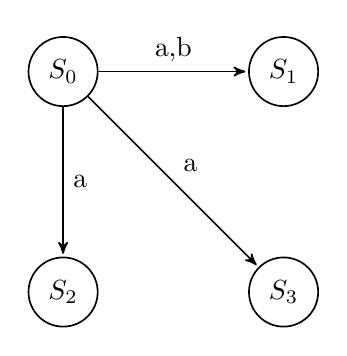
\begin{tikzpicture}[->,>=stealth',shorten >=1pt,auto,node distance=2.8cm,
                    semithick]
  \tikzstyle{every state}=[fill=none,draw=black,text=black]

  \node[state] (A) {$S_0$};
  \node[state] (R) [right of =A] {$S_1$};
  \node[state] (D) [below of =A] {$S_2$};
  \node[state] (U) [right of =D] {$S_3$};

  \path (A) edge node {a,b} (R)
  			edge node {a} (D)
  			edge node {a} (U);
\end{tikzpicture}
\end{center}

This is a nice example of the idea of taking a non-deterministic FSA and turning it into a deterministic FSA. Notice that this is non-deterministic because we have two edges labeled $a$ out of $S_0$, the initial state, and we also have two edges labeled $b$ out of $S_0$, the initial state. We need to construct a FSA that only has 1 edge labeled $a$ and 1 edge labeled $b$ out of that state. The solution is to create new states that are actually the power set of the original states $\mathcal{S}$. With such a system of states, we can now include just a single edge leaving $S_0$ going to a state $S_{1,2}$ which represents the state containing the original $S_1$ and $S_2$. We can also create a state $S_{1,3}$ representing two states from the original diagram as a single state. And just by doing this, we have encoded this without duplicate labels on edges going out of one vertex of $\mathcal{M}$, the directed graph. Notice also that in the worst case, if we start with $n$ different states in $\mathcal{S}$, we could end up with $2^n$ states in the DFA. We could potentially need a new state for every possible combination of different states, and that would be equivalent to the power set of $\mathcal{S}$, which has size $2^n$. 


\begin{center}
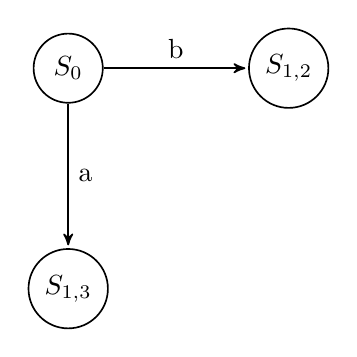
\begin{tikzpicture}[->,>=stealth',shorten >=1pt,auto,node distance=2.8cm,
                    semithick]
  \tikzstyle{every state}=[fill=none,draw=black,text=black]

  \node[state] (A) {$S_0$};
  \node[state] (R) [right of =A] {$S_{1,2}$};
  \node[state] (D) [below of =A] {$S_{1,3}$};

  \path (A) edge node {b} (R)
  			edge node {a} (D);
\end{tikzpicture}
\end{center}

In order to consider $\epsilon$ edges in our graph, we refer to Meier again \cite{ggt}. In the proof involving $\epsilon$ edges, first we construct a graph $\mathcal{M}_\epsilon$ which contains no edges labeled with an $\epsilon$. The states of $\mathcal{M}_\epsilon$ are the $\epsilon$-closed subsets of $V(\mathcal{M}$. The way the graph's edges are defined is as follows (from Groups, Graphs, and Trees)\cite{ggt}: For every $a\in \mathcal{S}$, the letters in the alphabet for $\mathcal{M}$, and a state $S$ of $\mathcal{M}_\epsilon$ (which is a subset $S\subset V(\mathcal{M})$ that is $\epsilon$-closed), consider every edge labeled $a$ that starts from a vertex in $S$, and let $Sa$ be the set of all states that are at the ends of such edges in $\mathcal{M}$. Then we take $\epsilon(Sa)$ and let there be an edge labeled $a$ from $S$ to $\epsilon(Sa)$. Additionally, define start states to be all $S$ that contain a start state, and accept states to be all $S$ that contain an accept state. The way our edges are defined guarantees that there are no edges labeled with $\epsilon$ in this new graph $\mathcal{M}_\epsilon$. 

Given this process of converting any non-deterministic automaton $\mathcal{M}$ into $\mathcal{M}_\epsilon$ with no edges labeled with $\epsilon$, we can now apply the process we showed in the earlier example; that is, create states for each possible combination of existing states, and let an edge denote that from $S_x$ to $S_y$, labeled $a$, where $x$ and $y$ are combinations of states in the original graph $\mathcal{M}_\epsilon$, there are edges labeled with $a$ in $\mathcal{M}_\epsilon$ from all the vertices in $x$ to all the vertices in $y$. Thus, we've shown any non-deterministic automaton can be converted into a deterministic FSA with the same accepted language (which is now a regular language). So we have thus shown containment both ways, and we have proved Theorem 7.12!

One important fact that needs to be stated is that \emph{not all languages are regular.} Deeply encoded into this notion is the idea of whether a language would need an infinite amount of memory to determine if a word is in the language. This notion is represented by the very important Pumping Lemma.

\textbf{Pumping Lemma}: Let $\mathcal{L}$ be a regular language. Then there is an integer $n\geq 1$ such that any word $x\in \mathcal{L}$ of length greater than $n$ can be expressed as $x=uvw$ where $v$ is a non-empty word, and:
\begin{enumerate}
\item $|u|<n$;
\item $uv^iw\in \mathcal{L}$ for all $i\geq 0$.
\end{enumerate}

We should definitely go over the key concepts of the proof of this important lemma. The way that Meier takes $n$ in this proof is to let it be at most equal to the number of vertices $V(\mathcal{M})$. Then, we know that any word in $\mathcal{L}$ must include some cycle from a vertex to itself again (We have to traverse some vertex twice, and in doing so must have a loop). We have the term $i$ to represent the number of times the cycle is traversed. We know, then, that taking just $uw$ with absolutely no cycles would be equivalent to having any number of cycles - thus we know that $uv^iw\in \mathcal{L}$ for all $i\geq 0$. To quote Meier, "the only difference in the paths is how many times they wind around the closed path"\cite{ggt}! 

One of the goals in our project is to show that the language $\{a^nb^n|n\in \N\}$ is not a regular language. It turns out that the Pumping Lemma is key to approaching this proof. In fact, the proof is actually quite simple given the Pumping Lemma. What we do is fix an $n=V(\mathcal{M})$ (showing that the FSA is in fact finite). We assume $\mathcal{L}$ is regular, and use proof by contradiction. Take $a^{n+1}$, which, since it is longer than $n$ length, has a closed loop of length $k$. We can write, then, that $a^{n+1+k}b^{n+1}$ is a word accepted by $\mathcal{L}$, where in reality we know $n+1+k\neq n+1$. In words, we know that $a^{n+1}b^{n+1}$ is accepted, and the Pumping Lemma states then that given that closed path of length $k$ we could add another such path in the middle. Additionally, this path comes out of the $a^x$ part of the word, as $a^{n+1}$ has length greater than $n$. So we can add another $v$ to the path to make $uv^2w$ which corresponds to $a^{n+1+k}b^{n+1}$ which shouldn't be accepted but is. Since $\mathcal{L}$ violates the Pumping Lemma, it cannot be regular! And thus we've gotten at least one example of a language that's not regular, namely $\{a^nb^n|n\geq 1\}$. To supplement, Farb gives an explanation that a finite state automaton has no memory, and in this case cannot "remember" how many $b$'s to accept after having accepted some amount of $a$'s \cite{farb}.

We now move towards the understanding of how FSA can be applied to group theory in the form of \emph{automatic groups}. First we need to understand the motivation for studying automatic groups. There are quite a few given by Farb. One motivation is solving the word problem - automatic groups have solvable word problems. Another is the "Cayley graph described by linear recursion", which was formalized by Thurston by using - you guessed it - finite state automata (FSA)! \cite{farb}. It turns out that FSA are great for studying normal forms of groups (as we looked at earlier in this paper), and automatic groups can be defined using only FSA.

A useful idea is the \emph{two-variable padded language}. We will compare two words at a time when working with automatic group, and it is useful for these words to be paired letter with letter. For example, given words $u$ and $v$ (notation that we will use throughout the rest of the paper), $u=u_1u_2\cdots u_n$ and $v=v_1v_2\cdots v_m$. For whichever of $n$ and $m$ is smaller, we will pad $u$ or $v$ respectively with \$ signs until $u,v$ have the same length - so that we can interpret two words with $(u_1,v_1),(u_2,v_2)\cdots(u_{m+1},\$)\cdots(u_n,\$)$ (if $v$ were longer, we'd have the \$ in the $u$-positions). We slightly redefine some of the language-related concepts to accommodate this new padding concept. 

Our first concept to redefine is the FSA $\mathcal{M}$ itself. To show that we include the padding symbol \$, we use the new alphabet, $\mathcal{S}\cup \$$. Since we now work with pairs of words instead of single words, our vertices must be labeled by pairs of letters from the alphabet $\mathcal{S}\cup\$$, which looks like $(\mathcal{S}\cup\$)\times (\mathcal{S}\cup \$) \ (\$,\$)$ (We do not include the pair (\$,\$) because we would not pad both words; only the shorter gets padded). Then, the vertices must be labeled not with letters in the alphabet $\mathcal{S}\cup \$$, but rather, with ordered pairs, once again like $(\mathcal{S}\cup\$)\times (\mathcal{S}\cup \$) \ (\$,\$)$. Now that we have redefined our directed graph for the FSA $\mathcal{M}$, we can redefine the concept of \emph{accepted language}. A language is now accepted by our FSA $\mathcal{M}$, if in $\mathcal{M}$ we read all the edges by $(u_1,v_1)\cdots$ and end up at an accept state in $\mathcal{M}$. Farb calls this \emph{regular over the padded alphabet} $\mathcal{S}$\cite{farb}. Farb also introduces an idea that the point of padding is that pairs of words can be read at "equal speeds" regardless of the lengths (which I believe is a more computer-science based property).

To actually define an automatic group, we choose a group and an alphabet. Let $G$ be the group with finite generating set $\mathcal{S}=\{s_1,s_2\cdots,s_n\}$. Additionally, instead of just choosing the generators, let $\mathcal{S}$ include a finite generating set $S$ and also all the inverses of the elements, $S^{-1}$. Then $\mathcal{S}=S\cup S^{-1}$. Farb defines a natural mapping here, from a free monoid $\mathcal{S}*$ to $G$, by taking any word $w$ to the group element it represents, call this map $w \mapsto \bar{w}$. Finally we get to define \emph{automatic groups}: $G$ is an automatic group if (and I paraphrase Farb here):
\begin{enumerate}
\item There is a language $\mathcal{L}$ over $\mathcal{S}$ given by FSA $\mathcal{M}$ such that the natural map we defined, call it $\pi: \mathcal{L}\rightarrow G$ is surjective (every $g\in G$ has some word in the language that maps to it). Let the image $\pi(w)$ is $\bar{w}$. We call $\mathcal{M}$ the \emph{word acceptor}. Having such a word acceptor allows us to define a normal form (which Farb calls a canonical form) for each $g\in G$.
\item The following languages are regular (accepted by $\mathcal{M}$):
\[\mathcal{L}_= = \{(u,v): u,v \in \mathcal{L} \& \bar{u}=\bar{v}\}\]
\[\mathcal{L}_{s_1} = \{(u,v): u,v \in \mathcal{L} \& \bar{u}=\overline{vs_1}\}\]
\[\vdots\]
\[\mathcal{L}_{s_n} = \{(u,v): u,v \in \mathcal{L} \& \bar{u}=\overline{vs_n}\}\].
\end{enumerate}
where $s_1,\cdots,s_n$ is all the generators in $\mathcal{S}$. $\mathcal{M}_=$ is the FSA which checks if $u,v$ are equivalent words (they both map to the same $g\in G$). Then, for each $s_i\in \mathcal{S}$, $\mathcal{M}_{s_i}$ is the FSA called the \emph{word comparator} \cite{farb}. 

Farb defines the collections of FSA's $\mathcal{M}, \mathcal{M}_=, \cdots, \mathcal{M}_{s_n}$ an \emph{automatic structure} for $G$. Here, we study an example of an automatic group: $\Z$, with respect to the generating set $\mathcal{S}=\{s,S=a^{-1}\}$. For this example, we will need 4 FSA: $\mathcal{M}, \mathcal{M}_=, \mathcal{M}_s, \mathcal{M}_S$. 

First we create the FSA $\mathcal{M}$:

\begin{center}
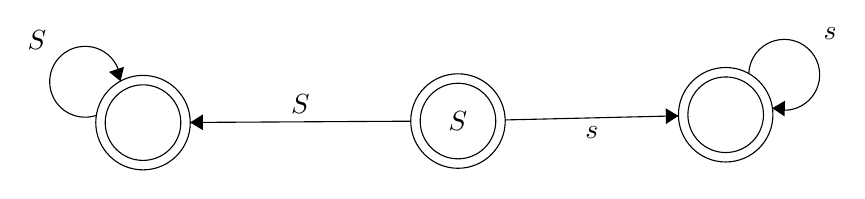
\begin{tikzpicture}[scale=0.2]
\tikzstyle{every node}+=[inner sep=0pt]
\draw [black] (37,-26.4) circle (3);
\draw (37,-26.4) node {$S$};
\draw [black] (37,-26.4) circle (2.4);
\draw [black] (54,-26) circle (3);
\draw [black] (54,-26) circle (2.4);
\draw [black] (17,-26.5) circle (3);
\draw [black] (17,-26.5) circle (2.4);
\draw [black] (40,-26.33) -- (51,-26.07);
\fill [black] (51,-26.07) -- (50.19,-25.59) -- (50.21,-26.59);
\draw (45.51,-26.72) node [below] {$s$};
\draw [black] (34,-26.41) -- (20,-26.49);
\fill [black] (20,-26.49) -- (20.8,-26.98) -- (20.8,-25.98);
\draw (27,-25.94) node [above] {$S$};
\draw [black] (14.048,-26.035) arc (288.78241:0.78241:2.25);
\draw (10.89,-21.24) node [left] {$S$};
\fill [black] (15.57,-23.87) -- (15.79,-22.96) -- (14.84,-23.28);
\draw [black] (55.469,-23.398) arc (178.28688:-109.71312:2.25);
\draw (60.18,-20.85) node [right] {$s$};
\fill [black] (56.96,-25.58) -- (57.74,-26.11) -- (57.77,-25.11);
\end{tikzpicture}
\end{center}

Then we create $\mathcal{M}_=$, which differs from $\mathcal{M}$ in that it is labeled by pairs of points to compare words, not just show the language:

\begin{center}
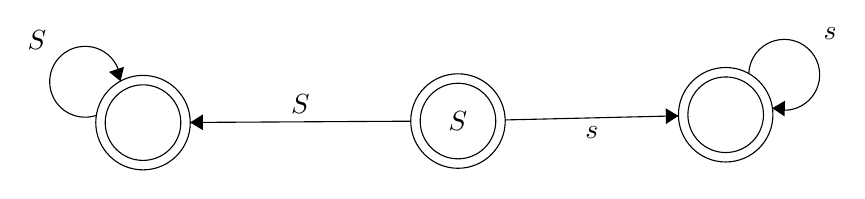
\begin{tikzpicture}[scale=0.2]
\tikzstyle{every node}+=[inner sep=0pt]
\draw [black] (37,-26.4) circle (3);
\draw (37,-26.4) node {$S$};
\draw [black] (37,-26.4) circle (2.4);
\draw [black] (54,-26) circle (3);
\draw [black] (54,-26) circle (2.4);
\draw [black] (17,-26.5) circle (3);
\draw [black] (17,-26.5) circle (2.4);
\draw [black] (40,-26.33) -- (51,-26.07);
\fill [black] (51,-26.07) -- (50.19,-25.59) -- (50.21,-26.59);
\draw (45.51,-26.72) node [below] {$s$};
\draw [black] (34,-26.41) -- (20,-26.49);
\fill [black] (20,-26.49) -- (20.8,-26.98) -- (20.8,-25.98);
\draw (27,-25.94) node [above] {$S$};
\draw [black] (14.048,-26.035) arc (288.78241:0.78241:2.25);
\draw (10.89,-21.24) node [left] {$S$};
\fill [black] (15.57,-23.87) -- (15.79,-22.96) -- (14.84,-23.28);
\draw [black] (55.469,-23.398) arc (178.28688:-109.71312:2.25);
\draw (60.18,-20.85) node [right] {$s$};
\fill [black] (56.96,-25.58) -- (57.74,-26.11) -- (57.77,-25.11);
\end{tikzpicture}
\end{center}

\newpage
Next is the comparator $\mathcal{M}_s$:

\begin{center}
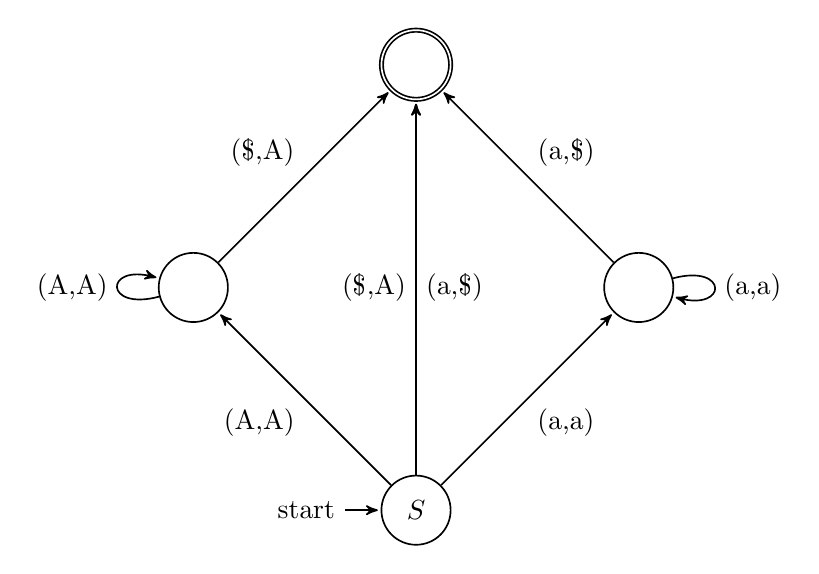
\begin{tikzpicture}[->,>=stealth',shorten >=1pt,auto,node distance=4cm,
                    semithick]
  \tikzstyle{every state}=[fill=none,draw=black,text=black]

  \node[state] (A)                    {};
  \node[state, accepting]         (B) [above right of=A] {};
  \node[initial,state]         (D) [below right of=A] {$S$};
  \node[state]         (C) [below right of=B] {};

  \path (A) edge              node {(\$,A)} (B)
            edge [loop left]  node {(A,A)}  (A)
        (D) edge [xshift=-1ex]node {(\$,A)} (B)
        	edge [xshift=1ex] node [right] {(a,\$)} (B)
        	edge              node {(A,A)}  (A)
        	edge              node [below right] {(a,a)}  (C)
        (C) edge [loop right] node {(a,a)}  (C)
        	edge              node [above right] {(a,\$)} (B);
\end{tikzpicture}
\end{center}

And finally we have the comparator $\mathcal{M}_{S}$:

\begin{center}
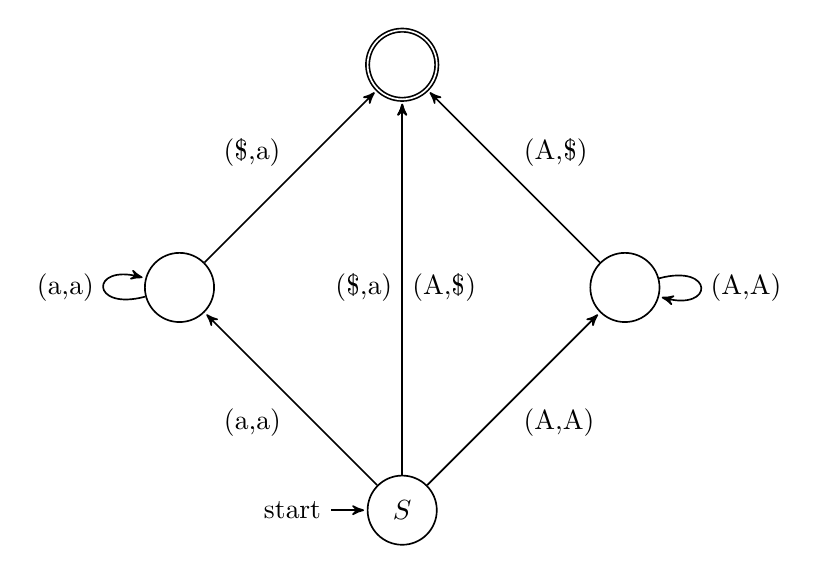
\begin{tikzpicture}[->,>=stealth',shorten >=1pt,auto,node distance=4cm,
                    semithick]
  \tikzstyle{every state}=[fill=none,draw=black,text=black]

  \node[state] (A)                    {};
  \node[state, accepting]         (B) [above right of=A] {};
  \node[initial,state]         (D) [below right of=A] {$S$};
  \node[state]         (C) [below right of=B] {};

  \path (A) edge              node {(\$,a)} (B)
            edge [loop left]  node {(a,a)}  (A)
        (D) edge [xshift=-1ex]node {(\$,a)} (B)
        	edge [xshift=1ex] node [right] {(A,\$)} (B)
        	edge              node {(a,a)}  (A)
        	edge              node [below right] {(A,A)}  (C)
        (C) edge [loop right] node {(A,A)}  (C)
        	edge              node [above right] {(A,\$)} (B);
\end{tikzpicture}
\end{center}

Since we are able to create the automatic structure for $\Z$, and we are able to create the language for $\Z$, $\Z$ is an automatic group\cite{farb}!

At this point, armed with our definition of an automatic group and an example of how to construct an example word comparator, we can discuss different examples of automatic groups! First of all, finite groups are automatic. The easiest rationale for this is that we can easily construct a FSA for each of the generators in $G$ (all finite groups must be finitely generated), and we can construct an FSA namely because there are a limited number of elements in $G$ and therefore a limited number of maximum possible states for each FSA. Thus, we can create the word comparator for each generator in $G$, and by our definition of automatic group, $G$ is automatic if it is finite. Another example (a bit more interesting than finite groups) is $\Z$, which we have just shown by construction; by creating the languages and the automatic structure we show that $\Z$ satisfies our definition and must be automatic. 

Yet another interesting example arises from the the free group of rank 2 (generators $a,b$), which is also automatic. We can construct the FSA for the language, $\mathcal{M}$ given $a,b$ and their inverses $A=a^{-1},B=b^{-1}$: 

\begin{center}
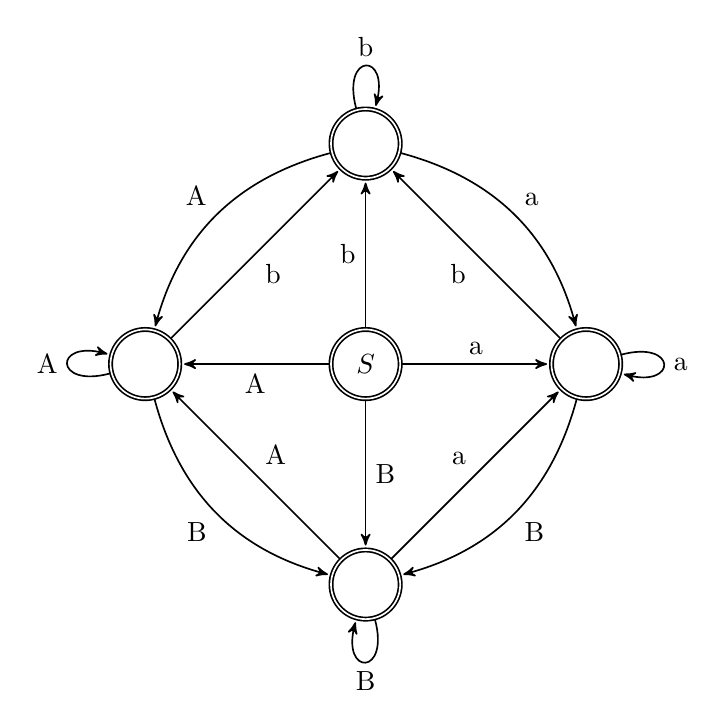
\begin{tikzpicture}[->,>=stealth',shorten >=1pt,auto,node distance=2.8cm,
                    semithick]
  \tikzstyle{every state}=[fill=none,draw=black,text=black]

  \node[state,accepting] (A) {$S$};
  \node[state,accepting] (L) [left of =A] {};
  \node[state,accepting] (R) [right of =A] {};
  \node[state,accepting] (U) [above of =A] {};
  \node[state,accepting] (D) [below of =A] {};

  \path (A) edge node {b} (U)
  			edge node {a} (R)
  			edge node {A} (L)
  			edge node {B} (D)
  		(D) edge [loop below] node {B} (D)
  			edge node [above right] {A} (L) 
  			edge node [above left] {a} (R)
  		(L) edge [loop left] node {A} (L)
   			edge [bend right] node [below left] {B} (D)
        	edge node [below right] {b} (U)
        (R) edge [loop right] node {a} (R)
        	edge [bend left] node [below right] {B} (D)
        	edge node [below left] {b} (U)
        (U) edge [bend right] node [above left] {A} (L)
        	edge [loop above] node {b} (U)
        	edge [bend left] node [above right] {a} (R);
\end{tikzpicture}
\end{center}

It's fairly easy to create the $\mathcal{M}_=$ comparator for the graph as well:

\begin{center}
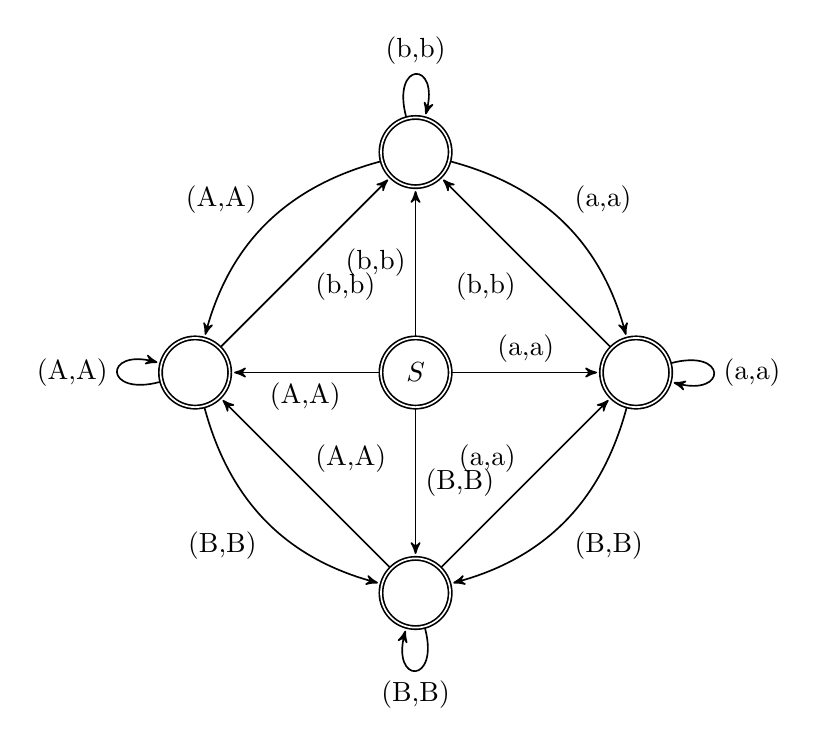
\begin{tikzpicture}[->,>=stealth',shorten >=1pt,auto,node distance=2.8cm,
                    semithick]
  \tikzstyle{every state}=[fill=none,draw=black,text=black]

  \node[state,accepting] (A) {$S$};
  \node[state,accepting] (L) [left of =A] {};
  \node[state,accepting] (R) [right of =A] {};
  \node[state,accepting] (U) [above of =A] {};
  \node[state,accepting] (D) [below of =A] {};

  \path (A) edge node {(b,b)} (U)
  			edge node {(a,a)} (R)
  			edge node {(A,A)} (L)
  			edge node {(B,B)} (D)
  		(D) edge [loop below] node {(B,B)} (D)
  			edge node [above right] {(A,A)} (L) 
  			edge node [above left] {(a,a)} (R)
  		(L) edge [loop left] node {(A,A)} (L)
   			edge [bend right] node [below left] {(B,B)} (D)
        	edge node [below right] {(b,b)} (U)
        (R) edge [loop right] node {(a,a)} (R)
        	edge [bend left] node [below right] {(B,B)} (D)
        	edge node [below left] {(b,b)} (U)
        (U) edge [bend right] node [above left] {(A,A)} (L)
        	edge [loop above] node {(b,b)} (U)
        	edge [bend left] node [above right] {(a,a)} (R);
\end{tikzpicture}
\end{center}

It would take 4 comparators $\mathcal{M}_a,\mathcal{M}_b,\mathcal{M}_A,\mathcal{M}_B$ to create the entire automatic structure, so I'll just create $|mathcal{M}_a$; notice that we can just view $a$ as $a^{-1},b,b^{-1}$ and create a similar FSA for each. 

\begin{center}
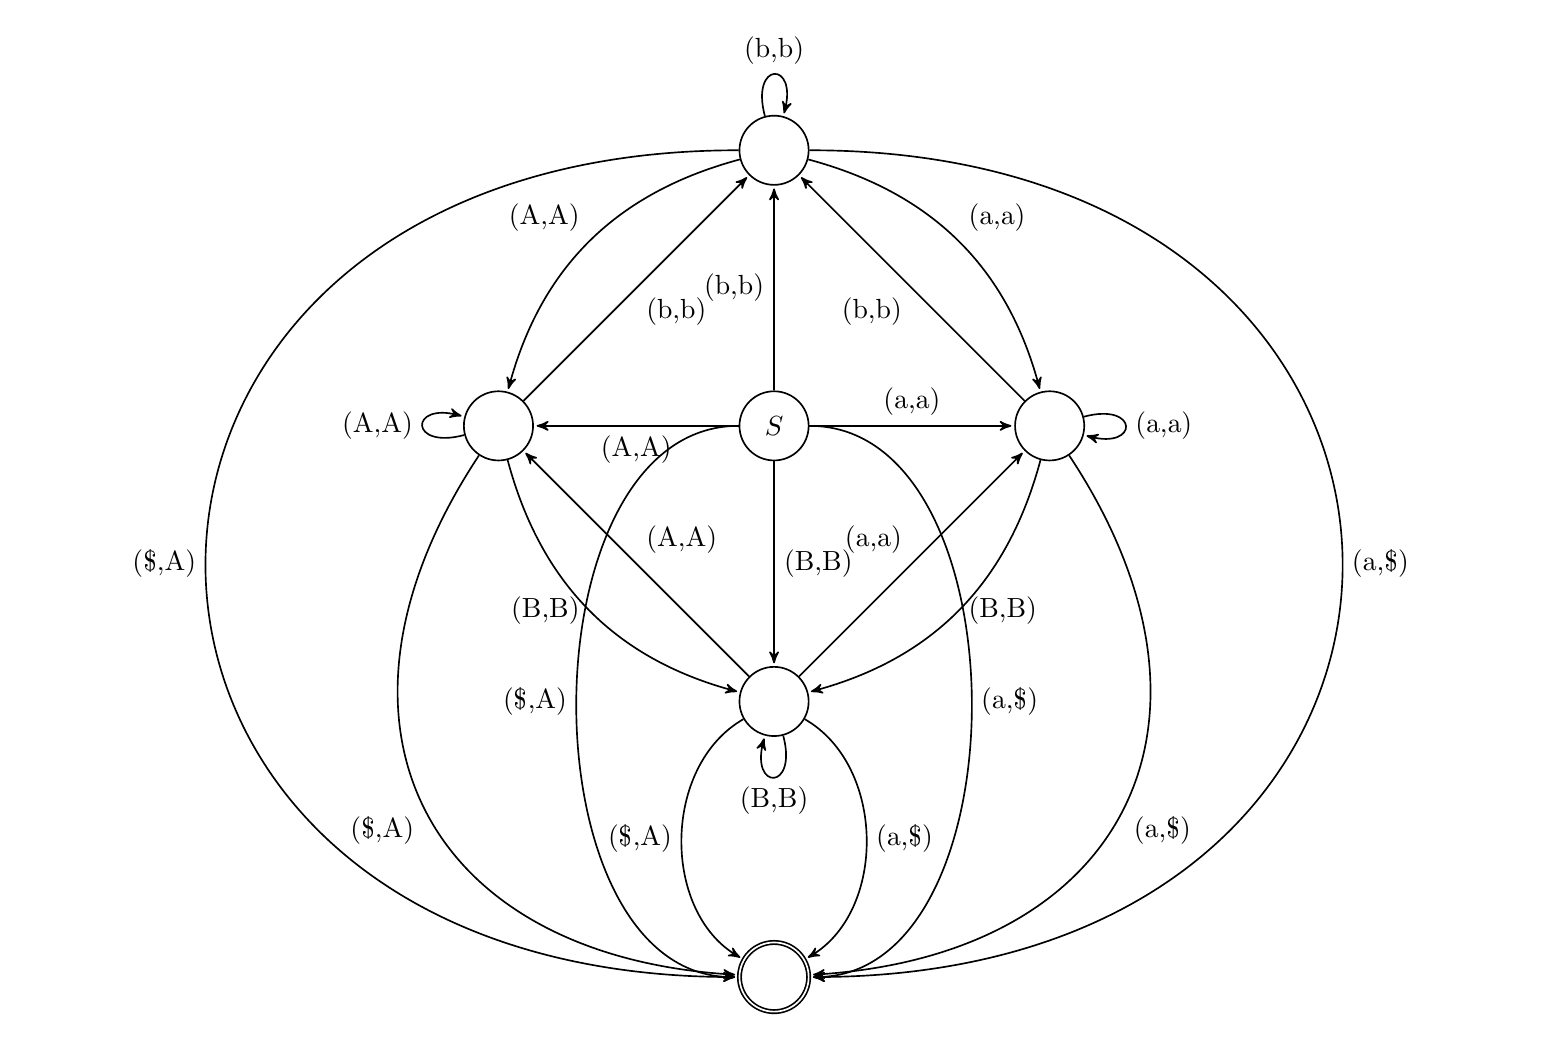
\begin{tikzpicture}[->,>=stealth',shorten >=1pt,auto,node distance=3.5cm,
                    semithick]
  \tikzstyle{every state}=[fill=none,draw=black,text=black]

  \node[state] (A) {$S$};
  \node[state] (L) [left of =A] {};
  \node[state] (R) [right of =A] {};
  \node[state] (U) [above of =A] {};
  \node[state] (D) [below of =A] {};
  \node[state,accepting] (F) [below of =D] {};

  \path (A) edge node {(b,b)} (U)
  			edge node {(a,a)} (R)
  			edge node {(A,A)} (L)
  			edge node {(B,B)} (D)
  			edge [bend left=90] node [right] {(a,\$)} (F)
  			edge [bend right=90] node [left] {(\$,A)} (F)
   		(D) edge [loop below] node {(B,B)} (D)
  			edge node [above right] {(A,A)} (L) 
  			edge node [above left] {(a,a)} (R)
  			edge [bend left=60] node [right] {(a,\$)} (F)
  			edge [bend right=60] node [left] {(\$,A)} (F)
  		(L) edge [loop left] node {(A,A)} (L)
   			edge [bend right] node [left] {(B,B)} (D)
        	edge node [below right] {(b,b)} (U)
        	edge [bend right=60, looseness=1.4] node [below left] {(\$,A)} (F)
        (R) edge [loop right] node {(a,a)} (R)
        	edge [bend left] node [right] {(B,B)} (D)
        	edge node [below left] {(b,b)} (U)
        	edge [bend left=60, looseness=1.4] node [below right] {(a,\$)} (F)
        (U) edge [bend right] node [above left] {(A,A)} (L)
        	edge [loop above] node {(b,b)} (U)
        	edge [bend left] node [above right] {(a,a)} (R)
        	edge [bend left=90, looseness=2.2] node [right] {(a,\$)} (F)
  			edge [bend right=90, looseness=2.2] node [left] {(\$,A)} (F);
\end{tikzpicture}
\end{center}

Note that in a free group, for 2 elements to differ by a single generator by right-multiplication is to guarantee that all elements to the left of the last value are identical. Therefore, much of this graph is derived from the previous equality checker. (Apologies for the amount of crossing, but I determined that there is no good way to draw this without some amount of intersections).

We can introduce an alternative definition of the automatic group, which involves the definition of the $k$\emph{-fellow traveler property.} and is more heavily geometric and gives us more insight to properties of the Cayley graph. The definition of the $k$-fellow traveler property is as follows: $d_{\Gamma_s(G)}(u(t),v(t))\leq k$ for all $t\geq 0$\cite{farb}. That is, as we traverse two paths, regardless of their length, we can define a constant $k$ such that the distance between the two points on the two paths is always less than or equal to $k$. 

With this definition, we can now state our alternate definition (quoting Farb): A group $G$ is automatic iff the following properties hold:
\begin{enumerate}
\item $G$ has a word acceptor $\mathcal{M}$ with regular language $\mathcal{L}(\mathcal{M})$ over some finite generating set $\mathcal{S}$, with the language and alphabet (generating set) satisfying all the properties we discussed in the first condition of our first definition.
\item There is a constant $k$ such that if $u,v\in \mathcal{L}(\mathcal{M})$ represents elements of $G$ which are distance 1 apart in $\Gamma_\mathcal{S}(G)$, then the paths $u$ and $v$ satisfy the $k$-fellow traveler property.
\end{enumerate}

In words, this means that the first condition is the same, but there is an equivalence between the second conditions. having the padded languages $\mathcal{L}_{s_1}\cdots \mathcal{L}_{s_n}$ be regular, or having a word comparator for each generator, is equivalent to stating that any paths in the Cayley graph can be at most $k$ distance apart. This is a very surprising fact! One must keep in mind that for the most part, the groups being studied are infinite, and for very long paths $u,v$, to have $\bar{u},\bar{v}$ differ by a generator seems not to guarantee \emph{anything} about the distance while stepping along the two paths. I felt that this result is so striking that it's necessary to go over the concepts of the proofs in both directions.

Direction 1: Given we have the automatic structure and all the word comparators for a group $G$, we can prove that $u,v$ paths in $\Gamma_\mathcal{S}(G)$ where $\bar{u},\bar{v}$ are distance 1 apart, they satisfy the $k$-fellow traveler property. Let a constant $c$ be an integer larger than the number of states in the FSA with the most states in the automatic structure of $G$. We do this in order to guarantee that there is a path of length less than $c$ in some FSA that leads to an accept state! That means that we can apply a path of at most $c-1$ (less than $c$) to get these states to either be equal, or be a generator apart, which is length 1. Then, the distance between $\overline{u(t)}$ and $\overline{v(t)}$, where $\bar{u},\bar{v}$ are the paths, and $\bar{u(t)},\bar{v(t)}$ are some point while traversing the paths $u$ and $v$. We see, then, that the total length of the path between the actual points is $2(c-1)+1$, because we have 1 path of length $c-1$ for $\overline{u(t)}$ and another path of length $c-1$ for $\overline{v(t)}$, and as previously discussed, they could be at most a generator apart depending on which word comparator we are using, which adds a length of 1. So the value of $k$ is $k=2(c-1)+1=2c-1$. And thus, definition 1 implies definition 2 for automatic groups.

Direction 2: Given the $k$-fellow traveler property for $u,v\in \mathcal{L}(\mathcal{M})$ in $\Gamma_\mathcal{S}(G)$, where $\bar{u},\bar{v}$ are a distance 1 part, we can construct the word comparators that make up the automatic structure for $G$. The idea here is to build a new FSA called \emph{Diff} of which we then take parts to build the comparators $\mathcal{M}_=,\mathcal{M}_{s_1}\cdots \mathcal{M}_{s_n}$. Define the states of this \emph{Diff} to be $S \times S \times B_k$, where $S$ is the set of states in the word acceptor $\mathcal{M}$ and $s_0$ is the start state \cite{farb}. \emph{Diff}, if at a point $(s_1,s_2,g)$, is fed the movements $(x,y)$, goes to $(t_1,t_2,x^{-1}gy)$, signifying that there was originally a path $g$, but by tracing the path backwards on $x$, then going across with $g$, then going forward on $y$, we can go between these two paths (with a length of at most $k$. So the real path between $t_1,t_2$ should be a path equivalent to the process we just described!

Essentially, \emph{Diff} \cite{farb} can become an FSA that keeps track of whether two paths are accepted by $\mathcal{M}$ and how far away the two paths are. We can derive the automatic structure and all the word acceptors from \emph{Diff} alone - by taking the accept states $(s_1,s_2,a_i)$ as the accept states of \emph{Diff}, we can create $\mathcal{M}_{a_i}$. To create $\mathcal{M}_=$, we use $e$ as the third position to find the accept states we should have. So we are able to create the automatic structure and all word acceptors simply by knowing the $k$-fellow traveler property.

The implications of these two definitions is probably the most interesting conclusion, geometrically speaking. Farb introduced the idea of 'linear recursion' formalized in the form of automatic structure and finite state automata, but now we see that the $k$-fellow traveler property proves that the Cayley graph $\Gamma_\mathcal{S}(G)$ is determined by the $k$-ball around the identity and further parts of the Cayley graph are simply copies of the ball of radius $k$ centered around the identity, pieced together by the automatic structure. And this final tying together of the automatic group's structure in terms of FSAs and the geometric structure in terms of the $k$-fellow traveler property and the Cayley Graph represents the interlocking and interwoven aspect of group theory that Farb is looking to highlight \cite{farb}.

In conclusion, we looked at the concept of Finite State Automata, the concepts of languages, both regular and not regular and how they relate to FSA. We used these definitions to create the concept of an automatic group using only FSA, and gave examples of constructions of an automatic structure for an automatic group. Finally, we showed an alternative, geometric definition was equivalent to the FSA-based definition, and this allowed us to get geometric insight into how the Cayley graph of an automatic group could be formed and defined.



\bibliographystyle{plain}	
\bibliography{refs}


\end{document} 